\apendice{Validación experimental}

Esta sección va a tener 2 tipos de test.
Uno primero evalúa la calidad del procesado y análisis en términos  de líneas extraídas y como se corresponden estás con las líneas reales en cuento al número de pixels .
Y un segundo test más avanzado va a comparar las propiedades de las lineas extraidas por la aplicación con las extraidas manualmente.

\section{Test de calidad mediante matriz de confusión}

En esta parte vamos a evaluar la calidad del proceso de binarización, esqueletizado, extracción de lineas y combinación de segmentos en términos de medidas obtenidas a partir de la matriz de confusión.
En dicha matriz un pixel representado como línea es un positivo y el fondo es negativo. Hay por lo tanto cuatro opciones: <<True Positive (TP),False Positive (FP), True Negative (TN), False Negative (FN)>> como podemos observar en la tabla \ref{tab:ConfMatrix}.

En este apartado vamos a mostrar las medidas que vamos a usar para conseguir la calidad de las imágenes y explicar las formulas obtenidas de \cite{wiki:confMatrix}.

Este primer test evalúa que las lineas reales se correspondan con líneas extraídas, pero no tiene en cuenta el número ni longitud de estas.

\begin{itemize}
\item True positive rate (TPR): Mide la proporción de los elementos que se han considerado como positivos y son positivos.
\[\mathit{TPR}=\frac{\mathit{TP}}{\mathit{TP}+\mathit{FN}}\]

\item True negative rate (TNR):Mide la proporción de los elementos que se han considerado como negativos y son negativos. 
\[\mathit{TNR}=\frac{\mathit{TN}}{\mathit{FP}+\mathit{TN}}\]

\item Positive predictive value (PPV): Mide la proporción de elementos clasificados como verdaderos positivos entre los positivos.
\[\mathit{PPV}=\frac{\mathit{TP}}{\mathit{TP}+\mathit{FP}}\]


\item Negative predictive value (NPV): Mide la proporción de elementos clasificados como verdaderos negativos entre los negativos.  
\[\mathit{NPV}=\frac{\mathit{TN}}{\mathit{TN}+\mathit{FN}}\]


\item False positive rate (FPR):
Mide la proporción de los elementos que se han considerado como falsos positivos entre los que son negativos reales.
 \[\mathit{FPR}=1-\mathit{TNR}\]

\item False discovery rate (FDR):
Mide la proporción de los elementos que se han considerado como falsos positivos entre los que son positivos de verdad.
\[\mathit{FDR}=1-\mathit{PPV}\]

\item Miss rate or false negative rate (FNR):
Mide la proporción de los elementos que se han considerado como falsos negativos entre los que son  positivos.
\[\mathit{FNR}=1-\mathit{TPR}\]

\item Accuracy (ACC): Mide el error observable.
\[\mathit{\mathit{ACC}}=\frac{\mathit{TP}+\mathit{TN}}{P+N}\]

\item Valor F1: Este valor muestra la media armónica entre la precision y la sensibilidad del modelo.
\[\mathit{F1}=\frac{2\mathit{TP}}{2\mathit{TP}+\mathit{FP}+\mathit{FN}}\]

\item Matthews correlation coefficient (MCC):
Esta medida se usa en Maching Learning para medir la calidad de la clasificación en dos clases \cite{wiki:machineMCC}.
 \[\mathit{MCC}=\frac{\mathit{TP}*\mathit{TN}-\mathit{FP}*\mathit{FN}}{\sqrt{(\mathit{TP}+\mathit{FP})*(\mathit{TP}+\mathit{FN})*(\mathit{TN}+\mathit{FP})*(\mathit{TN}+\mathit{FN})}}\]
 
\item Informedness or Bookmaker Informedness (BM):
Esta medida informa de la generalización de un problema multi-clases y estima la probabilidad de decisión.
 \[\mathit{BM}=\mathit{TPR}+\mathit{TNR}-1\]

\item Markedness (MK):
Esta es la medida de cuando una variable es marcada como predicción o causa posible de otra.
 \[\mathit{MK}=\mathit{PPV}+\mathit{NPV}-1\]


\end{itemize}



\subsection{Pruebas}
Aquí van a aparecer una muestra de las pruebas que hemos realizado sobre la aplicación para medir la calidad de la detección.


Para las pruebas vamos a optar por construir una matriz de confusion sobre los resultados, la tabla mostrada a continuación, sera el modelo que vamos a seguir \ref{tab:ConfMatrix}.

\begin{table}
  \begin{center}
    \begin{tabular}{c l c c}
                 &                & \multicolumn{2}{c}{\cellcolor{brown!25}Predicted condition}   \\
                 &                & \cellcolor{brown!15}Positive prediction & \cellcolor{brown!45}Negative prediction \\
       \cellcolor{blue!15}True      & \cellcolor{blue!10}Positive class & \cellcolor{green!25}True positive (TP)  & \cellcolor{red!25}False negative (FN) \\
       \cellcolor{blue!15}Condition & \cellcolor{blue!30}Negative class & \cellcolor{red!25}False positive (FP) & \cellcolor{green!25}True negative (TN)  \\
    \end{tabular}
  \end{center}
  \caption{Estructura de la matriz de confusion.}
  \label{tab:ConfMatrix}
\end{table}


La tabla en general va a contener las medidas que hemos mencionado anteriormente pero vamso a aclarar las medidas.
\begin{itemize}
\item Maximizar: TPR, TNR, PPV, NPV, ACC, F1, MCC, BM y MK.
Estas medidas se corresponden con el número de elementos que debemos maximizar ya que indican tanto aciertos en positivos como en falsos, pero aciertos.
\item Minimizar: FPR, FDR y FNR.
Estas medidas las cuanto menores sean será mejor ya que indicará que no fallamos ni en positivos ni en negativos.
\end{itemize}

Prueba 1: La matriz de confusión obtenida para esta prueba la podemos observar en la tabla \ref{tab:pruebas}.
Las imágenes original, como muestra la figura \ref{fig:orip1}, y calculada, como muestra la figura \ref{fig:calcp1}, las podemos observar en la figura \ref{fig:p1}.
Los resultados de las medidas de calidad se muestran en la tabla \ref{tab:parte}.

Prueba 2: La matriz de confusión obtenida para esta prueba la podemos observar en la tabla \ref{tab:pruebas}.
Las imágenes original, como muestra la figura \ref{fig:orip2}, y calculada, como muestra la figura \ref{fig:calcp2}, las podemos observar en la figura \ref{fig:p2}.
Los resultados de las medidas de calidad se muestran en la tabla \ref{tab:parte}.

Prueba 3: La matriz de confusión obtenida para esta prueba la podemos observar en la tabla \ref{tab:pruebas}.
Las imágenes original, como muestra la figura \ref{fig:orip3}, y calculada, como muestra la figura \ref{fig:calcp3}, las podemos observar en la figura \ref{fig:p3}.
Los resultados de las medidas de calidad se muestran en la tabla \ref{tab:parte}.

Prueba 4: La matriz de confusión obtenida para esta prueba la podemos observar en la tabla \ref{tab:pruebas}.
Las imágenes original, como muestra la figura \ref{fig:orip4}, y calculada, como muestra la figura \ref{fig:calcp4}, las podemos observar en la figura \ref{fig:p4}.
Los resultados de las medidas de calidad se muestran en la tabla \ref{tab:parte}.




\begin{table}[]
\centering
\caption{Tabla de resultados matriz de confusión}
\label{tab:pruebas}
\rowcolors {2}{gray!35}{}
\begin{tabular}{ lrrrr }
\toprule
Prueba                & True positive & False negative & False positive & True negative \\ \midrule
Figura \ref{fig:p1} & 36\,136         & 3\,840           & 3\,685           & 1\,185\,139       \\ 
Figura \ref{fig:p2} & 31\,670         & 844            & 6\,514           & 1\,189\,772       \\ 
Figura \ref{fig:p3} & 23\,114         & 8\,238           & 7\,103           & 1\,190\,345       \\ 
Figura \ref{fig:p4} & 30\,284         & 1\,773           & 14\,753          & 1\,181\,990       \\ \bottomrule
\end{tabular}
\end{table}



\begin{table}[]
\centering
\caption{Resultados medidas de calidad}
\label{tab:parte}
\rowcolors {2}{gray!35}{}
\resizebox{\textwidth}{!}{
\begin{tabular}{ lllllllllllllll }
\toprule
Prueba                & TPR$\uparrow$  & TNR$\uparrow$  & PPV$\uparrow$  & NPV$\uparrow$  & FPR$\downarrow$   & FDR$\downarrow$  & FNR$\downarrow$  & ACC$\uparrow$  & F1$\uparrow$   & MCC$\uparrow$  & BM$\uparrow$   & MK$\uparrow$   \\ \midrule
Figura \ref{fig:p1} & 0.90 & 0.99 & 0.99 & 0.99 & 0.003 & 0.09 & 0.09 & 0.99 & 0.91 & 0.90 & 0.9  & 0.90 \\ 
Figura \ref{fig:p2} & 0.97 & 0.99 & 0.83 & 0.99 & 0.17  & 0.17 & 0.02 & 0.99 & 0.90 & 0.90 & 0.83 & 0.82 \\ 
Figura \ref{fig:p3} & 0.74 & 0.99 & 0.76 & 0.99 & 0.01  & 0.24 & 0.26 & 0.99 & 0.75 & 0.74 & 0.73 & 0.76 \\ 
Figura \ref{fig:p4} & 0.94 & 0.99 & 0.67 & 0.99 & 0.01  & 0.33 & 0.05 & 0.99 & 0.78 & 0.79 & 0.93 & 0.67 \\ 
Media & 0.88 & 0.99 & 0.81 & 0.99 & 0.04  & 0.20 & 0.11 & 0.99 & 0.84 & 0.83 & 0.85 & 0.78 \\ 
Desviación & 0.10 & 0 & 0.13 & 0 & 0.08  & 0.10 & 0.10 & 0 & 0.08 & 0.08 & 0.08 & 0.09 \\ \bottomrule
\end{tabular}
}
\end{table}



\begin{figure}
	\begin{subfigure}[c]{.5\linewidth}
	\centering\large 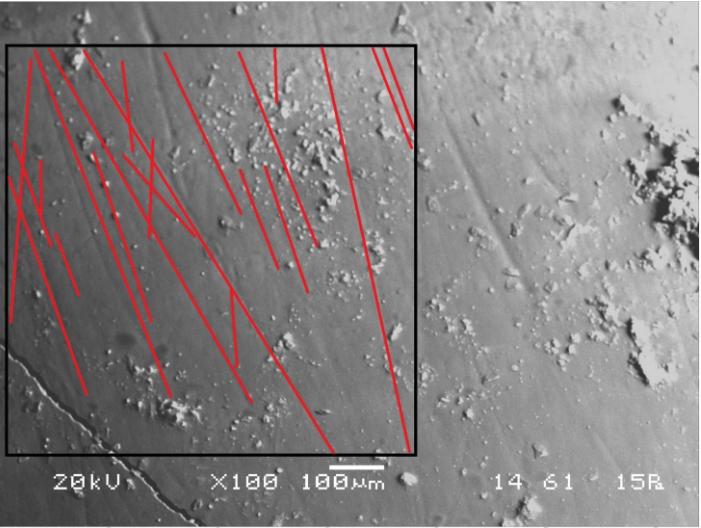
\includegraphics[width=.9\textwidth]{prueba1Ori}
	\caption{Estrías pintadas por el usuario.}\label{fig:orip1}
	\end{subfigure}%
	\begin{subfigure}[c]{.5\linewidth}
	\centering\large 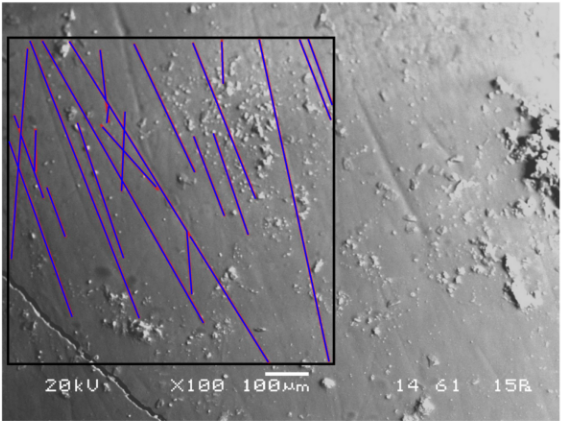
\includegraphics[width=.9\textwidth]{prueba1Detec}
	\caption{Estrías pintadas por la aplicacion.}\label{fig:calcp1}
	\end{subfigure}%
	\caption{Imágenes prueba 1}
	\label{fig:p1}
\end{figure}



\begin{figure}
	\begin{subfigure}[c]{.5\linewidth}
	\centering\large 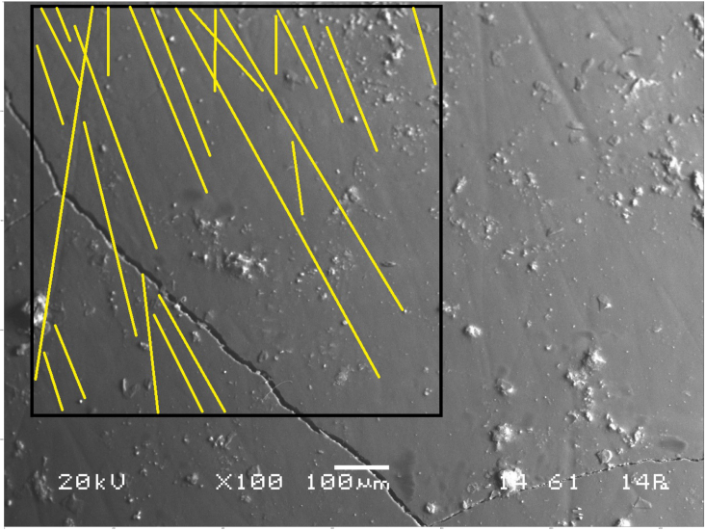
\includegraphics[width=.99\textwidth]{prueba2Ori}
	\caption{Estrías pintadas por el usuario.}\label{fig:orip2}
	\end{subfigure}%
	\begin{subfigure}[c]{.5\linewidth}
	\centering\large 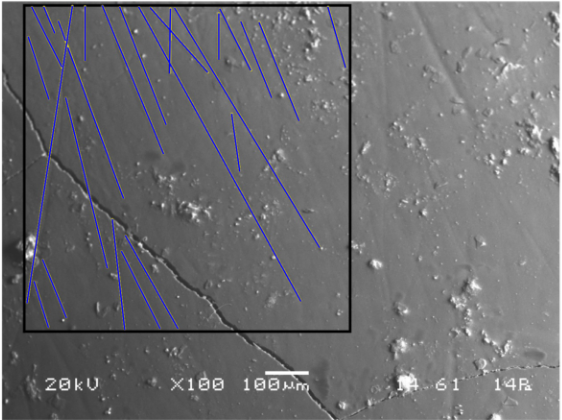
\includegraphics[width=.99\textwidth]{prueba2Detec}
	\caption{Estrías pintadas por la aplicacion.}\label{fig:calcp2}
	\end{subfigure}%
	\caption{Imágenes prueba 2}
	\label{fig:p2}

\end{figure}


\begin{figure}
	\begin{subfigure}[c]{.5\linewidth}
	\centering\large 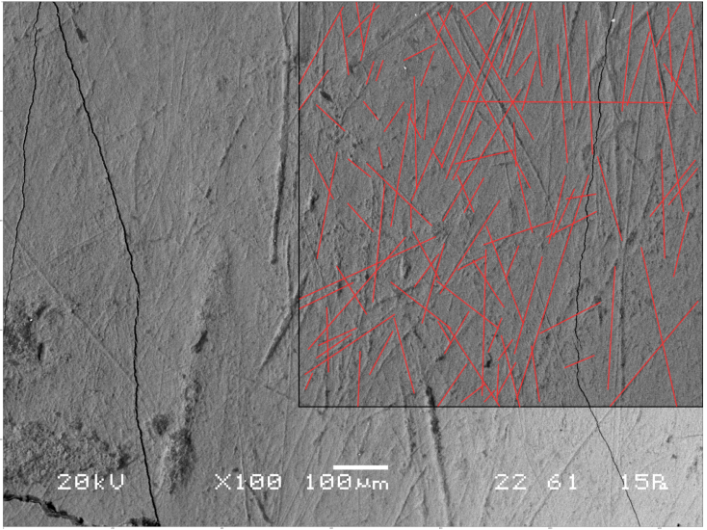
\includegraphics[width=.9\textwidth]{prueba3Ori}
	\caption{Estrías pintadas por el usuario.}\label{fig:orip3}
	\end{subfigure}%
	\begin{subfigure}[c]{.5\linewidth}
	\centering\large 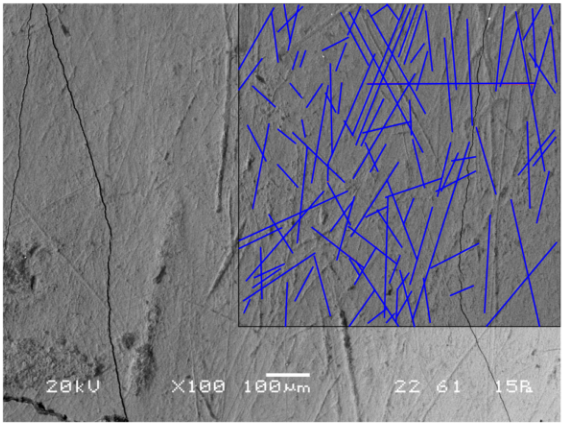
\includegraphics[width=.9\textwidth]{prueba3Detec}
	\caption{Estrías pintadas por la aplicacion.}\label{fig:calcp3}
	\end{subfigure}%
	\caption{Imágenes prueba 3}
	\label{fig:p3}

\end{figure}



\begin{figure}
	\begin{subfigure}[c]{.5\linewidth}
	\centering\large 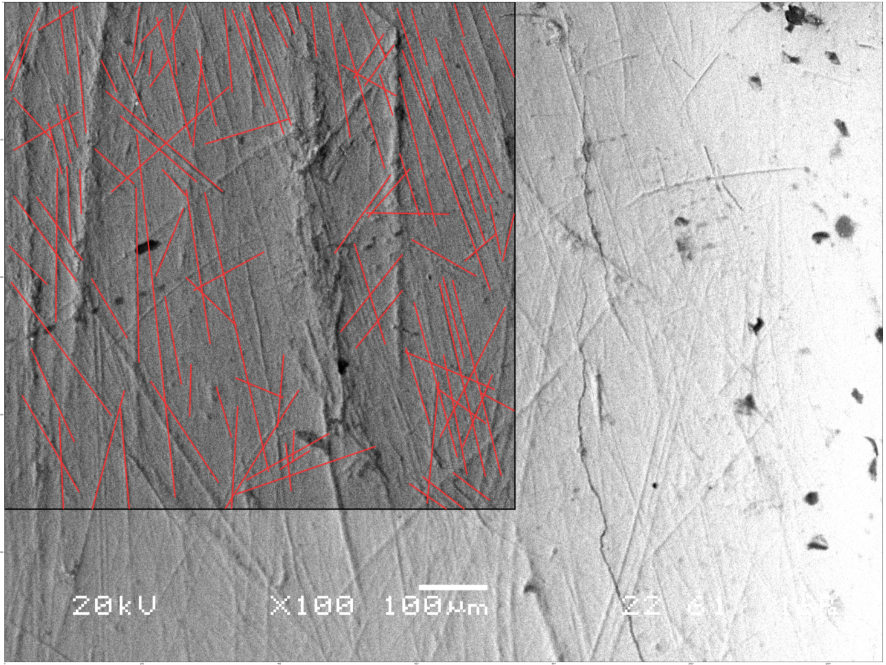
\includegraphics[width=.9\textwidth]{prueba4Ori}
	\caption{Estrías pintadas por el usuario.}\label{fig:orip4} 
	\end{subfigure}%
	\begin{subfigure}[c]{.5\linewidth}
	\centering\large 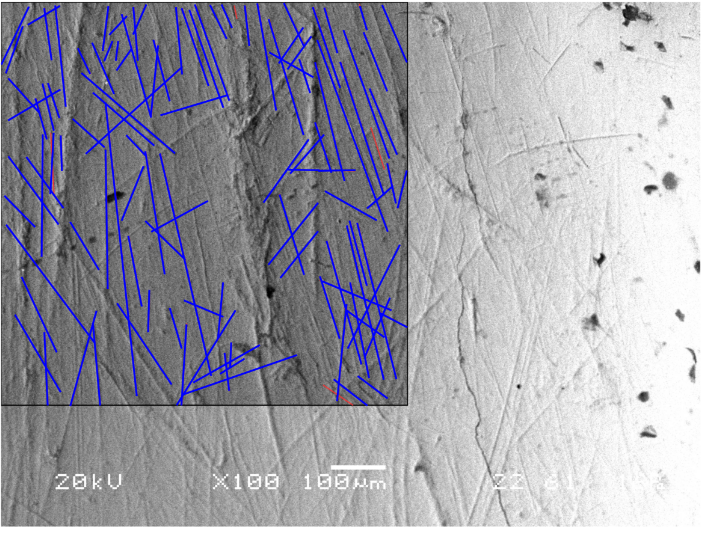
\includegraphics[width=.9\textwidth]{prueba4Detec}
	\caption{Estrías pintadas por la aplicacion.}\label{fig:calcp4}
	\end{subfigure}%
	\caption{Imágenes prueba 4}
	\label{fig:p4}

\end{figure}

\section{Test t de Student sobre las propiedades de las lineas extraídas.}

Puede ocurrir que el solapamiento entre los segmentos detectados por la aplicación y las estrías dibujadas por el investigador sea muy alto, pero el número de lineas y su longitud media varié. Esto sucede cuando una misma estría aparece detectada mediante dos segmentos en la aplicación o dos estrías diferentes aparecen detectadas mediante un único segmento.

Este nuevo test nos va ayudar a detectar esos casos porque vamos a hacer pruebas con los resultados obtenidos a mano por nuestros testers de la aplicación y los resultados obtenidos por nuestra aplicación, para ello vamos a hacer <<el test t de Student \cite{wiki:testStude}>>
Hay dos tipos de test t de student. El apareado o parejado y el despareado o de muestras independientes. El usado es el segundo.

Dicho test consiste en a partir de dos muestras comprar cuanta varia una de otra obteniendo un resultado entre 0 y 1. El resultado obtenido se puede evaluar de dos modos:
\begin{itemize}
\item Normal: Si el resultado obtenido es mayor de 0,05 significa que las muestras son parecidas y que pasan el test de Student menos estricto.
\item Estricto: Si el resultado obtenido es mayor o igual a 0.1 quiere decir que las dos muestras de población son prácticamente la misma ya que ha pasado el test de Student estricto.
\end{itemize} 

\begin{table}[]
\centering
\caption{Prueba t de Student realizada por Rebeca García \cite{Rebeca:garcia} y corregido por mi.}
\label{tab:estud}
\rowcolors {4}{gray!35}{}
\begin{tabular}{@{} lrrrrr @{}}
\toprule
\multirow{2}{*}{\textbf{Diente}} & \multicolumn{2}{l}{\textbf{Numero de estrías}} & \multicolumn{2}{l}{\textbf{Longitud promedio}} & \multirow{2}{*}{\textbf{Prueba \textit{t}}} \\ \cline{2-5}
                                 & \textbf{Automático}      & \textbf{Manual}     & \textbf{Automático}      & \textbf{Manual}     &                                    \\ \midrule
\textbf{7506-1}                  & 85,00                    & 80,00               & 339,76                   & 275,88              & 0,19                               \\ 
\textbf{7506-2}                  & 50,00                    & 55,00               & 269,17                   & 271,00              & 0,96                               \\ 
\textbf{7547-1}                  & 23,00                    & 21,00               & 300,00                   & 327,00              & 0,77                               \\ 
\textbf{7547-3}                  & 24,00                    & 24,00               & 263,70                   & 260,00              & 0,94                               \\ 
\textbf{7672-1}                  & 83,00                    & 75,00               & 202,77                   & 230,57              & 0,21                               \\ 
\textbf{7672-3}                  & 56,00                    & 52,00               & 211,93                   & 231,00              & 0,64                               \\ 
\textbf{7672B-1}                 & 65,00                    & 66,00               & 221,66                   & 233,00              & 0,64                               \\ 
\textbf{7672B-2}                 & 71,00                    & 69,00               & 215,86                   & 244,26              & 0,34                               \\ 
\textbf{7711-1}                  & 93,00                    & 76,00               & 195,07                   & 269,00              & 0,10                               \\ 
\textbf{7711-3}                  & 88,00                    & 80,00               & 188,71                   & 237,00              & 0,09                               \\ \bottomrule
\end{tabular}
\end{table}
Estos resultados se pueden encontrar los ficheros Excel originales en la carpeta <<Documentación-Archivos-Test de student>>